%Use one of the two documentclass lines depending on aspect ratio needed
% for 4x3 aspect ratio slides
%\documentclass{beamer}
%for 16x9 (modern wide screen) aspect ratio slides
%\documentclass[aspectratio=169]{beamer}
\documentclass[aspectratio=169]{beamer}
\usepackage{pifont}
\usepackage[normalem]{ulem}
\usepackage{booktabs}

% Oxford Maths theming
\usetheme{oxfordmaths}

% Set author etc info
\title[Belief Distribution Learning] %short version of title for slide footer
{
~\\
~\\
\large{Belief Distribution Learning - an extension to Evidential Deep Learning} 
~\\
~\\
~\\
~\\
} %full title for titlepage
\author{ Duncan Cameron-Steinke}
\institute{University of British Columbia, Okanagan Campus}
\date[Duncan C-S] {May 30, 2026}

%% Now for the actual slides %%
\begin{document}
\begin{frame}[plain]
  \titlepage
\end{frame}

\begin{frame}[t]
    \frametitle{What do these have in common?}
    
    \begin{columns}[t]
        \column{0.5\textwidth}
        \centering
        \textbf{States of a Hidden Markov Model}
        \vspace{0.5em}
        
        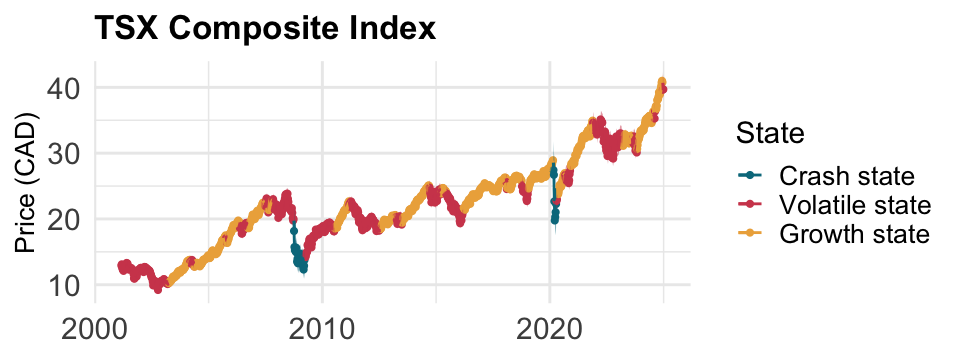
\includegraphics[width=0.9\linewidth]{intro_plots/hmm-timeseries.png}
        
        \column{0.5\textwidth}
        \centering
        \textbf{Facial Expressions}
        \vspace{0.5em}
        
        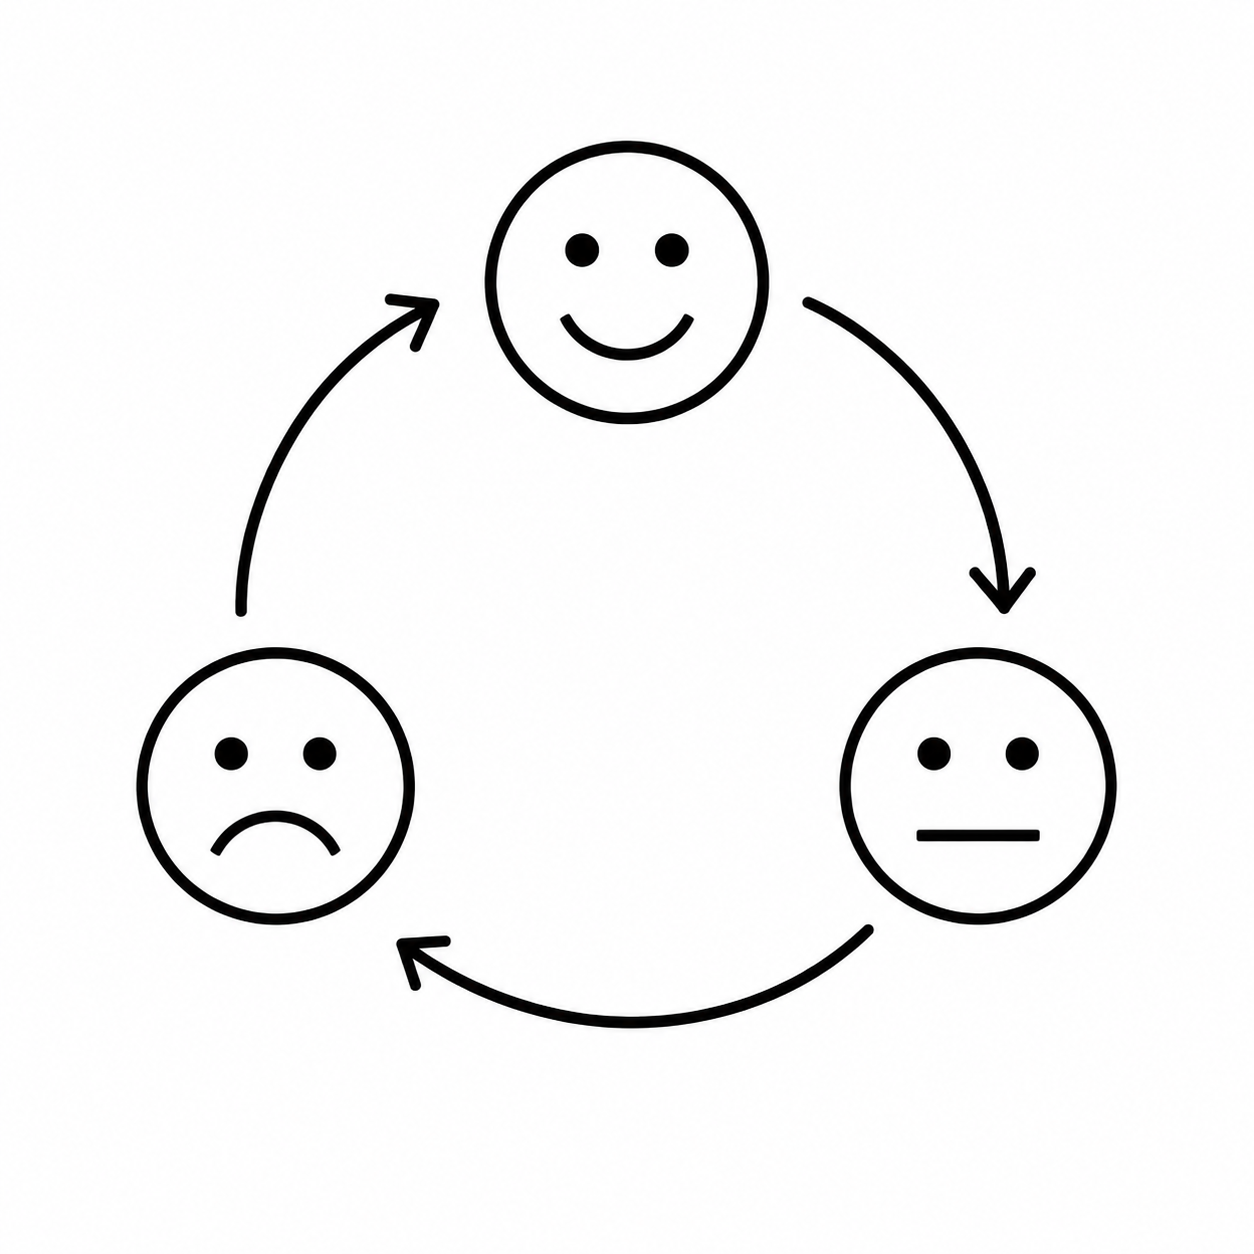
\includegraphics[width=0.35\linewidth]{intro_plots/facial emotions.png}
    \end{columns}
    
    \pause
    
    {\centering \textbf{They both represent Label Distribution Learning} \par}
    \vspace{1em}
    
    \begin{columns}[t]
        \column{0.5\textwidth}
        \centering
        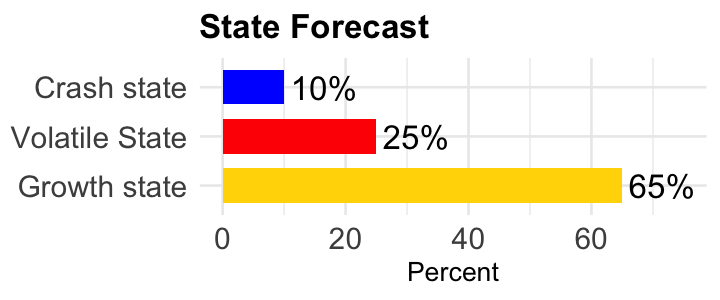
\includegraphics[width=0.8\linewidth]{intro_plots/hmm_state_label_dist.png}
        
        \column{0.5\textwidth}
        \centering
        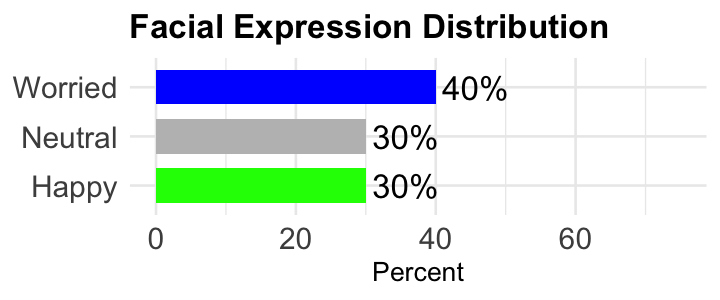
\includegraphics[width=0.8\linewidth]{intro_plots/facial emotions distribution.png}
    \end{columns}
\end{frame}


\begin{frame}[t]
    \frametitle{Research Goal}
    Develop an uncertainty aware Deep Learning classifier for LDL applications.
    \begin{itemize}
        \item Prioritize accuracy
        \item Provide calibrated uncertainty estimation
    \end{itemize}

    \begin{figure}
        \centering
        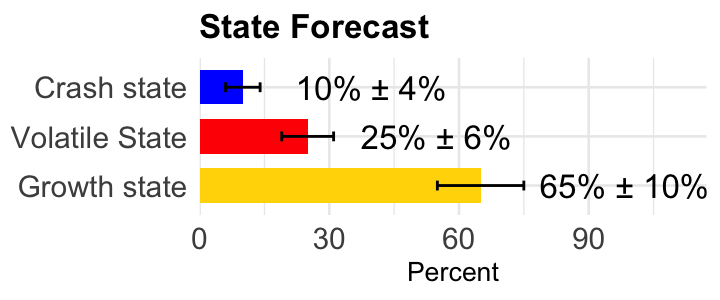
\includegraphics[width=0.5\linewidth]{intro_plots/hmm_state_label_dist_with_error.png}
        \label{fig:placeholder}
    \end{figure}
    
    
\end{frame}


\begin{frame}[T]
    \vfill
    \centering
    {\usebeamerfont{title}\usebeamercolor[fg]{title}\Large Generic Prediction \\ vs \\ Evidential Deep Learning\par}
    \vfill
\end{frame}

\begin{frame}[t]
    \frametitle{Generic Prediction}

    Softmax prediction output:
    \begin{figure}
        \centering
        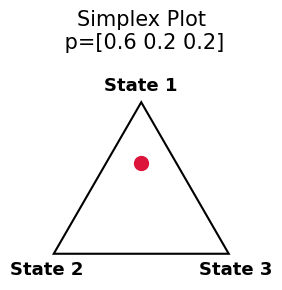
\includegraphics[width=0.3\linewidth]{evidential_deeplearning/simplex_plot.png}
        \caption{ Point estimate with no uncertainty prediction.}
        \label{fig:placeholder}
    \end{figure}
    
\end{frame}

\begin{frame}[t]
    \frametitle{Evidential Deep Learning}

    Dirichlet distribution output:
    \begin{figure}
        \centering
        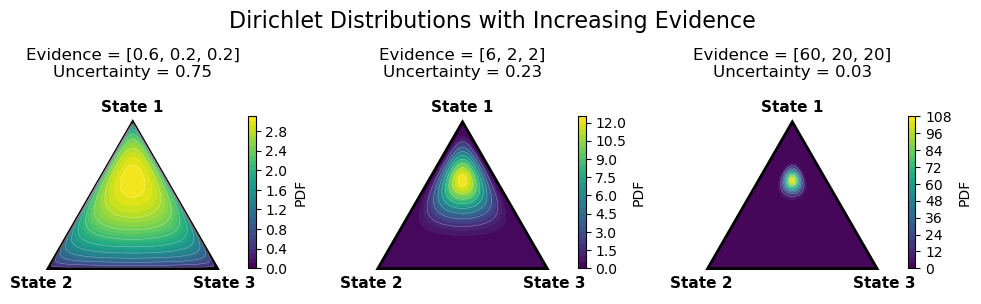
\includegraphics[width=0.9\linewidth]{evidential_deeplearning/dirichlet_sample_plots.png}
        \caption{Dirichlet distribution with uncertainty quantification.}
        \label{fig:placeholder}
    \end{figure}
    
\end{frame}


\begin{frame}[t]
    \frametitle{Evidential Deep Learning}
    In Evidential Deep Learning [Sensoy 2018], a neural network with a ReLU output layer learns an evidence vector $\mathbf{e}$ that parametrizes a Dirichlet Distribution.
    
    \vspace{0.5em}
    
    \textbf{Step 1:} The network maps inputs to evidence:
    \begin{equation}
        \mathbf{e} = f_{\hat\theta}(X) \qquad (\text{ReLU ensures } e_i \geq 0)
    \end{equation}

    
    \textbf{Step 2:} Evidence defines the Dirichlet parameters:
    \begin{align}
        \alpha_i &= e_i + 1 \quad \forall i \in K \\
        \text{Dir}(\mathbf{p}, \mathbf{\alpha}) &= \frac{1}{B(\alpha)}\prod_{i=1}^{K} p_i^{\alpha_i-1} \\
        \text{Model Uncertainty}: u &= \frac{K}{\sum_{i=1}^K \alpha_i}
    \end{align}
\end{frame}

\begin{frame}[t]{Evidential Deep Learning}
    \textbf{The Problem:} Learned evidence vectors treat each class independently and ignore the \emph{simplex constraint}.
    
    \vspace{2em}
    
    Because probabilities must sum to one, evidence towards one class \emph{requires} reduced evidence towards the other classes.
    
    \vspace{0.5em}
    
    \textbf{Example:} If the model is certain that $p_1 = 1$, then it must be equally certain that $p_2 = 0$, but standard EDL does not enforce this.
\end{frame}

\begin{frame}[T]
    \vfill
    \centering
    {\usebeamerfont{title}\usebeamercolor[fg]{title}\Large Belief Distribution Learning\par}
    \vfill
\end{frame}


\begin{frame}[t]{Belief Distribution Learning}
    Belief Distribution Learning is derived from \emph{Subjective Logic} [Jøsang 2016], which decomposes a probability into belief and uncertainty:
    
    \begin{align}
        \mathbf{P} &= \mathbf{b} + u\,\mathbf{a} \\
        1 &= u + \sum \mathbf{b}
    \end{align}
    
    \vspace{0.5em}
    
    where
    \begin{itemize}
        \item $\mathbf{b}$ — the \emph{belief} mass assigned to each outcome
        \item $u$ — the \emph{uncertainty} mass
        \item $\mathbf{a}$ — the \emph{base rate} (prior probability)
    \end{itemize}
    
    \vspace{0.5em}
    
    \begin{quote}
        The probability of an event is your \emph{belief}, plus your \emph{uncertainty} distributed according to the prior.
    \end{quote}
\end{frame}

\begin{frame}[t]{Belief Distribution Learning}
    We propose Belief Distribution Learning, where a deep learning model predicts the belief $\mathbf{b}$ and uncertainty $u$ through a \textbf{softmax} output layer.
    \begin{equation}
        u, \mathbf{b} = f_{\hat\theta}(X) \qquad \left(\text{Softmax ensures } \textstyle\sum b_i + u = 1\right)
    \end{equation}
    
    \vspace{0.75em}
    
    These outputs map to \textbf{Dirichlet parameters}, which provide uncertainty quantification:
    \begin{equation}
        \alpha_i = \frac{1}{K}\left( \frac{b_i}{u} + \bar{p}_i \right) + 1
    \end{equation}
    
    \vspace{0.5em}
    
    where $K$ is the number of classes, and $\bar{p}_i$ is the average class probability over the training data.
\end{frame}

\begin{frame}[t]{Belief Distribution Learning}
Example PDF plots
\begin{figure}
    \centering
    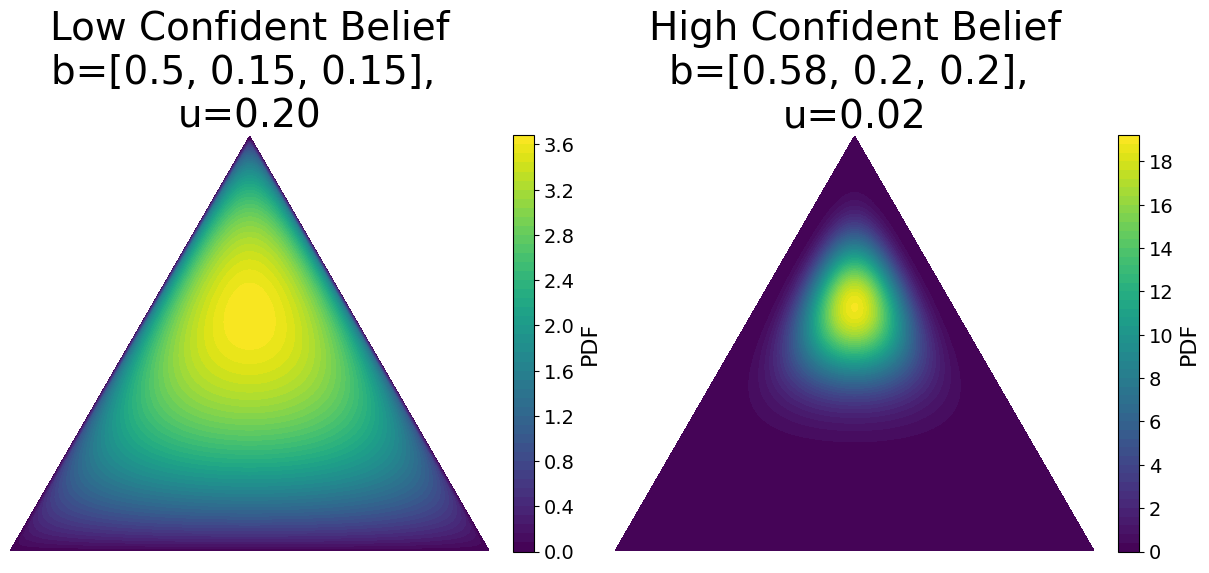
\includegraphics[width=0.5\linewidth]{evidential_deeplearning/BDL_sample.png}
    \caption{Sample low confidence and higher confidence predictions using Belief Distribution Learning.}
    \label{fig:placeholder}
\end{figure}
\end{frame}

\begin{frame}{BDL Results}
    \begin{table}
        \centering
        \caption{Label distribution prediction error on SJAFFE  dataset ($\downarrow$ lower is better)}
        \label{tab:sjaffe_accuracy}
        \begin{tabular}{lcccc}
            \toprule
            \textbf{Model} & \textbf{KL Div.} $\downarrow$ & \textbf{Chebyshev} $\downarrow$ & \textbf{Clark} $\downarrow$ & \textbf{Canberra} $\downarrow$\\
            \midrule
            \textbf{BDL}      & \textbf{0.042}$\pm$0.003 & \textbf{0.087}$\pm$0.004 & \textbf{0.319}$\pm$0.009 & \textbf{0.654}$\pm$0.019 \\
            EDL               & 0.053$\pm$0.004 & 0.103$\pm$0.004 & 0.357$\pm$0.010 & 0.741$\pm$0.023 \\
            DP & 0.073$\pm$0.004 & 0.119$\pm$0.005 & 0.424$\pm$0.012 & 0.886$\pm$0.026 \\
            SNEFY             & 0.136$\pm$0.011 & 0.146$\pm$0.007 & 0.566$\pm$0.021 & 1.172$\pm$0.044 \\
            \bottomrule
        \end{tabular}
    \end{table}
    
    \footnotesize
    \textbf{BDL} (ours): Belief Distribution Learning \quad
    \textbf{EDL}: Evidential Deep Learning [Sensoy 2018] \\
    \textbf{DP}: Direct Prediction \quad
    \textbf{SNEFY}: Squared Neural Family [Zhang 2025] \\
    
    \vspace{0.5em}
    \normalsize
    \textbf{Takeaway:} BDL achieves the lowest error across all four metrics.
\end{frame}
\begin{frame}[T]
    \vfill
    \centering
    {\usebeamerfont{title}\usebeamercolor[fg]{title}\Large multi-Belief Distribution Learning\par}
    \vfill
\end{frame}

\begin{frame}[t]{multi-Belief Distribution Learning}
    \textbf{The Idea:} What if we deconstruct multi label learning into K single label learners.
    \begin{itemize}
        \item Each learner is a 1 vs rest classifier
        \item The learners are constrained to the simplex using belief logic
    \end{itemize}
    \vspace{1em}
    From belief logic we define:
    \begin{align}
        p_i &= b_i + u_i \quad \forall i \in K \\
        1 &= \sum_{i=1}^K b_i + u_i\\
        \textbf{b, u} &= f_{\hat\theta}(X) \quad \left(\text{Softmax}\right)
    \end{align}
\end{frame}


\begin{frame}{Multi-Belief Distribution Learning}
    % Belief and uncertainty are predicted for \emph{each} label:
    
    \begin{center}
        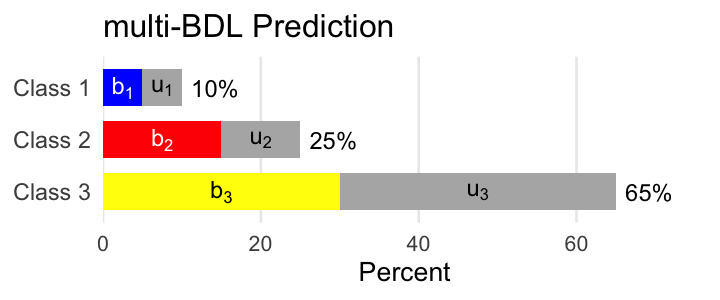
\includegraphics[width=0.45\linewidth]{evidential_deeplearning/mBDL-prediction.png}
    \end{center}
    
    \vspace{-0.5em}
    Construct $K$ Beta distributions (\textbf{one-vs-rest}):
    \begin{itemize}
        \setlength{\itemsep}{2pt}
        \item Class $i$: $\;\alpha_i = \frac{1}{K}\!\left(\frac{b_i + u_i}{u_i}\right) + 1$
        \item The rest: $\;\beta_i = \frac{1}{K}\!\left(\frac{1 - b_i - u_i}{u_i}\right) + 1$
    \end{itemize}
    
    The joint PDF is the product over labels:
    \vspace{-0.5em}
    \begin{equation*}
        \text{mBDL}(\mathbf{p} \mid \boldsymbol{\alpha}, \boldsymbol{\beta})
        = \prod_{i=1}^K \text{Beta}(p_i \mid \alpha_i, \beta_i)
    \end{equation*}
\end{frame}

\begin{frame}{Multi-Label Belief Distribution Learning}
    Multi-BDL has flexible confidence bounds while BDL does not.

    \begin{figure}
        \centering
        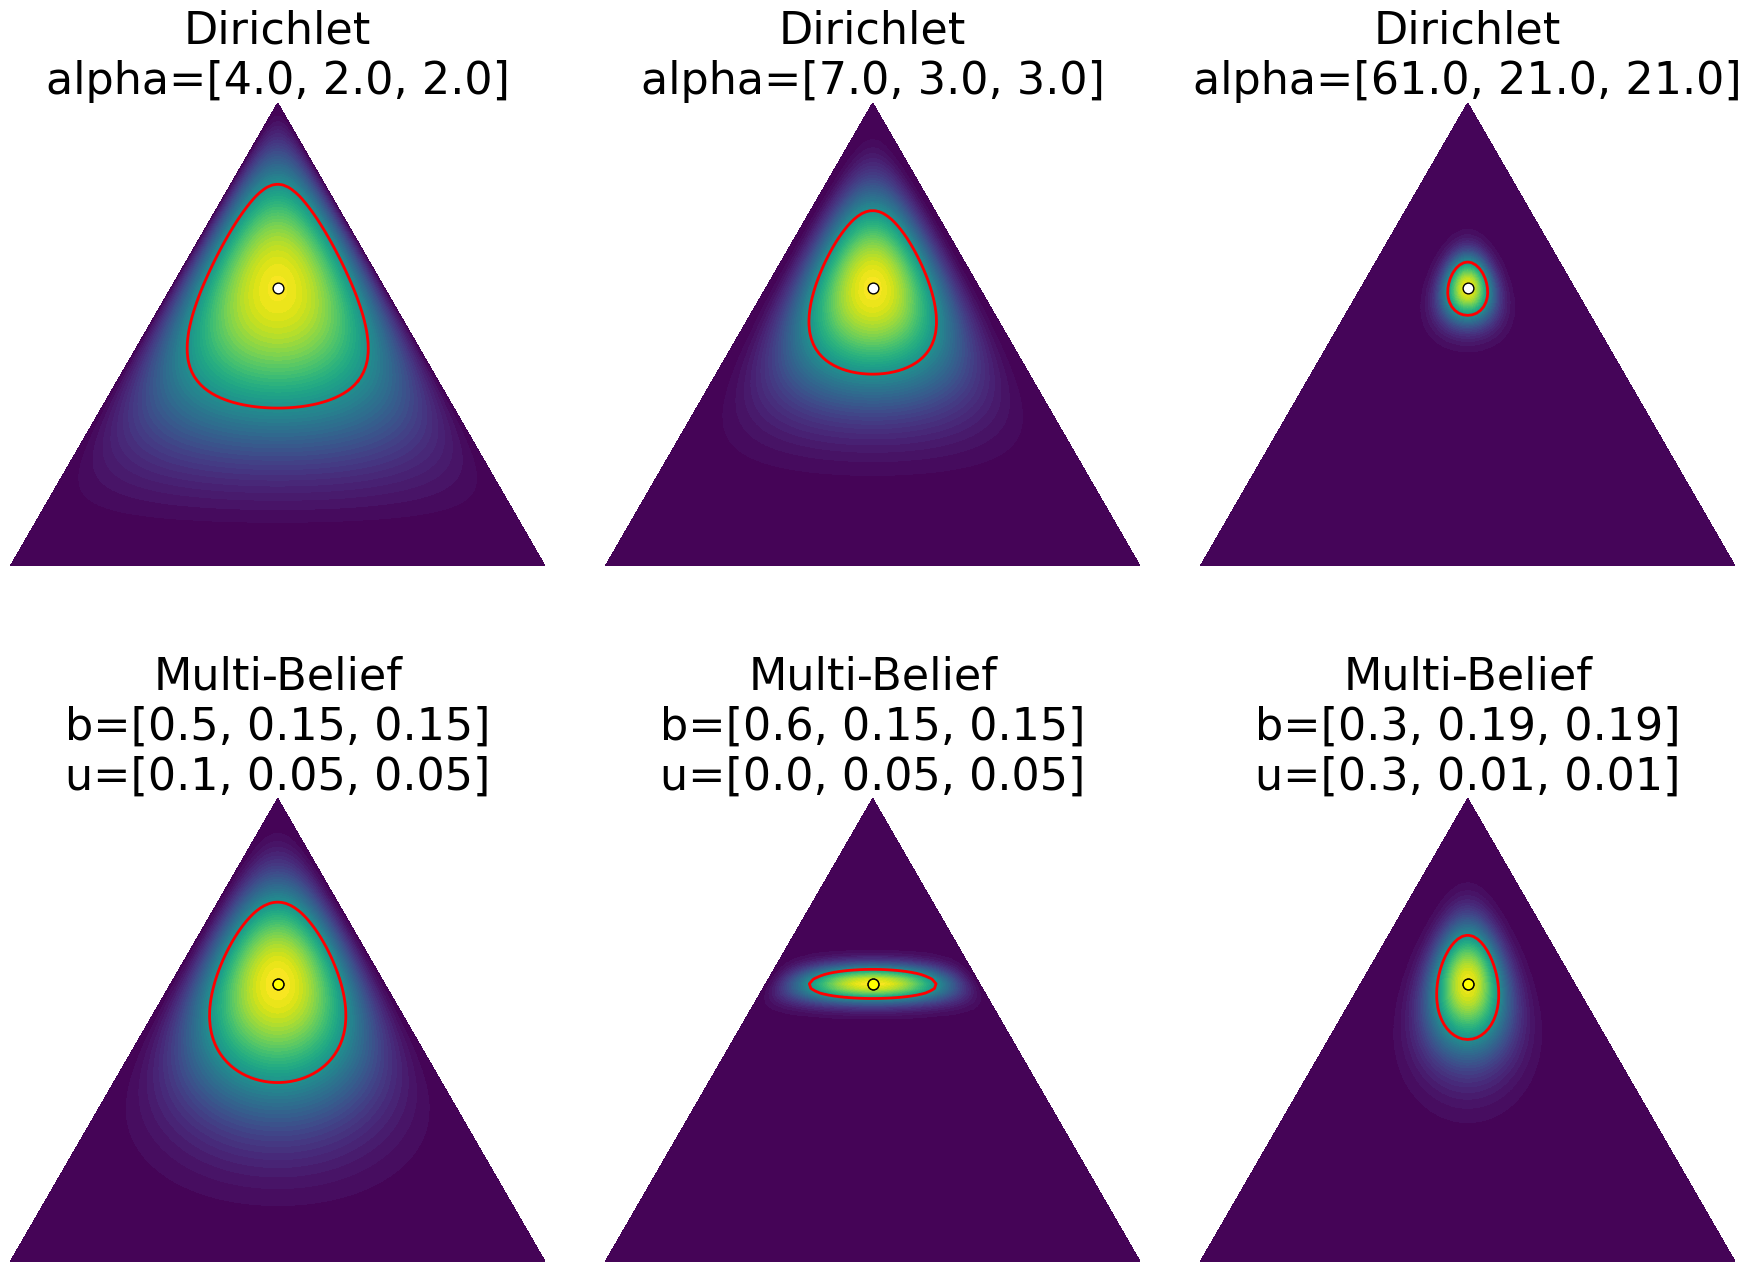
\includegraphics[width=0.55\linewidth]{evidential_deeplearning/mBDL_plots.png}
        \label{fig:placeholder}
    \end{figure}
\end{frame}

\begin{frame}{Results}
    \begin{table}
        \centering
        \caption{Label distribution error and conformal calibration on SJAFFE}
        \label{tab:sjaffe_results}
        \begin{tabular}{lccc}
            \toprule
            \textbf{Model} & \textbf{KL Div.} $\downarrow$ & \textbf{Joint FSC} $\uparrow$ & \textbf{Worst-Bin FSC} $\uparrow$ \\
            \midrule
            BDL              & \textbf{0.042}$\pm$0.003 & 0.551$\pm$0.034 & 0.518$\pm$0.039 \\
            \textbf{multiBDL} & \textbf{0.042}$\pm$0.002 & \textbf{0.586}$\pm$0.036 & \textbf{0.568}$\pm$0.030 \\
            EDL              & 0.060$\pm$0.005 & 0.510$\pm$0.034 & 0.488$\pm$0.022 \\
            DP               & 0.073$\pm$0.004 & 0.498$\pm$0.045 & 0.547$\pm$0.031 \\
            SNEFY            & 0.141$\pm$0.013 & 0.571$\pm$0.045 & 0.540$\pm$0.026 \\
            \bottomrule
        \end{tabular}
    \end{table}
    
    \footnotesize
    \textbf{KL Divergence:} Measure of agreement between predicted and true label distribution.
    \textbf{FSC (Feature-Stratified Coverage):} Uncertainty calibration metric. \\
    \textbf{Joint} Combined calibration across labels; \textbf{Worst-Bin} Worst performing quartiles across labels \\[0.3em]
    
    \vspace{0.5em}
    \normalsize
    \textbf{Takeaway:} multiBDL is equally accurate but much better calibrated.
\end{frame}

\begin{frame}[t]
    \frametitle{Conclusions}
    \begin{itemize}
        \item Belief theory from \textit{Subjective Logic} applied to the concepts of Evidential Deep Learning improves accuracy on LDL tasks.
        \item Multi-belied, which allows for label specific uncertainty, improves conformal predictions compared to competing methods.
    \end{itemize}
    
    \begin{table}
        \centering
        \label{tab:sjaffe_results}
        \begin{tabular}{lccc}
            \toprule
            \textbf{Model} & \textbf{KL Div.} $\downarrow$ & \textbf{Joint FSC} $\uparrow$ & \textbf{Worst-Bin FSC} $\uparrow$ \\
            \midrule
            BDL              & \textbf{0.042}$\pm$0.003 & 0.551$\pm$0.034 & 0.518$\pm$0.039 \\
            \textbf{multiBDL} & \textbf{0.042}$\pm$0.002 & \textbf{0.586}$\pm$0.036 & \textbf{0.568}$\pm$0.030 \\
            SNEFY            & 0.141$\pm$0.013 & 0.571$\pm$0.045 & 0.540$\pm$0.026 \\
            \bottomrule
        \end{tabular}
    \end{table}
\end{frame}


\begin{frame}[t]
    \frametitle{References}
    
    \textbf{Evidential Deep Learning to Quantify Classification Uncertainty}
    \vspace{0.2cm}
    
    \textbf{Author:} Murat Sensoy, Lance Kaplan, Melih Kandemir 
    \textbf{Proceedings:} 32nd Conference on Neural Information Processing Systems.
    \textbf{Year:} 2018 
    \vspace{0.5cm}
    
    \textbf{Label Distribution Learning using the Squared Neural Family on the Probability Simplex}
    \vspace{0.2cm}
    
    \textbf{Author:} Daokun Zhang, Russell Tsuchida, Dino Sejdinovic
    \textbf{Proceedings:} Forty-first Conference on Uncertainty in Artificial Intelligence.
    \textbf{Year:} 2025 
    \vspace{0.5cm}
    
    \textbf{Subjective Logic: A Formalism for Reasoning Under Uncertainty}
    \vspace{0.2cm}
    
    \textbf{Author:} Audun Jøsang
    \textbf{Publisher:} Springer, Artificial Intelligence: Foundations, Theory, and Algorithms series.
    \textbf{Year:} 2016
\end{frame}

\begin{frame}{Results on more datasets}

\begin{table}[h]
\centering
\caption{Accuracy and conformal metrics for SBU\_3DFE dataset}
\label{tab:sjaffe_sbu_accuracy}

\begin{tabular}{lcccc}
\toprule
\textbf{model} & \textbf{dataset} & \textbf{kl\_divergence} & \textbf{joint\_fsc} & \textbf{worst\_bin\_fsc} \\
\midrule
\texttt{EDL} & SBU\_3DFE & \textbf{0.067}±0.001 & 0.488±0.012 & 0.762±0.013 \\
\texttt{multiBDL} & SBU\_3DFE & \textbf{0.067}±0.001 & 0.482±0.013 & \textbf{0.790}±0.010 \\
\texttt{BDL} & SBU\_3DFE & 0.070±0.001 & 0.482±0.011 & 0.745±0.013 \\
\texttt{DP} & SBU\_3DFE & 0.076±0.001 & 0.480±0.008 & 0.765±0.007 \\
\texttt{SNEFY} & SBU\_3DFE & 0.409±0.050 & \textbf{0.575}±0.010 & 0.734±0.018 
\bottomrule
\end{tabular}

\end{table}
    
\end{frame}

\begin{frame}[t]
    \frametitle{Uncertainty types}
    \textbf{Epistemic Uncertainty}: When the model has insufficient information to make a confident prediction.
    \begin{itemize}
        \item[$\bullet$] Generally dominates in out-of-distribution examples.
        \item[$\circ$] Example: Covid-19 was a novel environment with high epistemic uncertainty.
        \item[$\rightarrow$] Predictions should have low confidence.
    \end{itemize}
   
    \textbf{Aleatoric Uncertainty}: Randomness inherent to the data itself.
    \begin{itemize}
        \item[$\bullet$] Should lead to more probability mass spread across the hidden states.
        \item[$\circ$] Example: Random week-to-week swings of an asset price.
        \item[$\rightarrow$] Predictions can have high confidence.
    \end{itemize}
\end{frame}



\end{document}
